	
No desenvolvimento de qualquer projeto, é essencial ter uma visão geral sobre as atividades que serão realizadas no decorrer da processo de criação.  Para isso existem formas de sistematização e organização dessas informações.

Uma dessas formas de organizar a informação é a EAP - Estrutra Analítica do Projeto - que é a estruturação das entregas a serem completadas em forma de árvore de maneira hierárquica, onde são distribuídas da mais gerais para as mais especificas.

A EAP foi a forma escolhida pela equipe de desenvolvimento do projeto EmerVant para estruturação das entregas, por proporcionar de uma maneira simples e objetiva todos os pontos abordados e discutidos para a realização do projeto em seu devidos graus de importância. 

Para a criação da EAP do EmerVant, foi observado que dentro do projeto há varias áreas de atuação. Assim os níveis mais gerais foram definidos por essas áreas de atuação que são:
\begin{itemize}
\item Gerência de Projetos;
\item Iniciação;
\item Estrutura do VANT;
\item Comunicação;
\item Controle;
\item Fonte Energética;
\item Encerramento.
\end{itemize}
As entregas especificas de cada tópico foram baseadas nas definições de escopo e requisitos. A Figura \ref{fig:eap} é a representação gráfica da EAP criada para o projeto EmerVant.
\begin{figure}[!h]
 \flushleft
    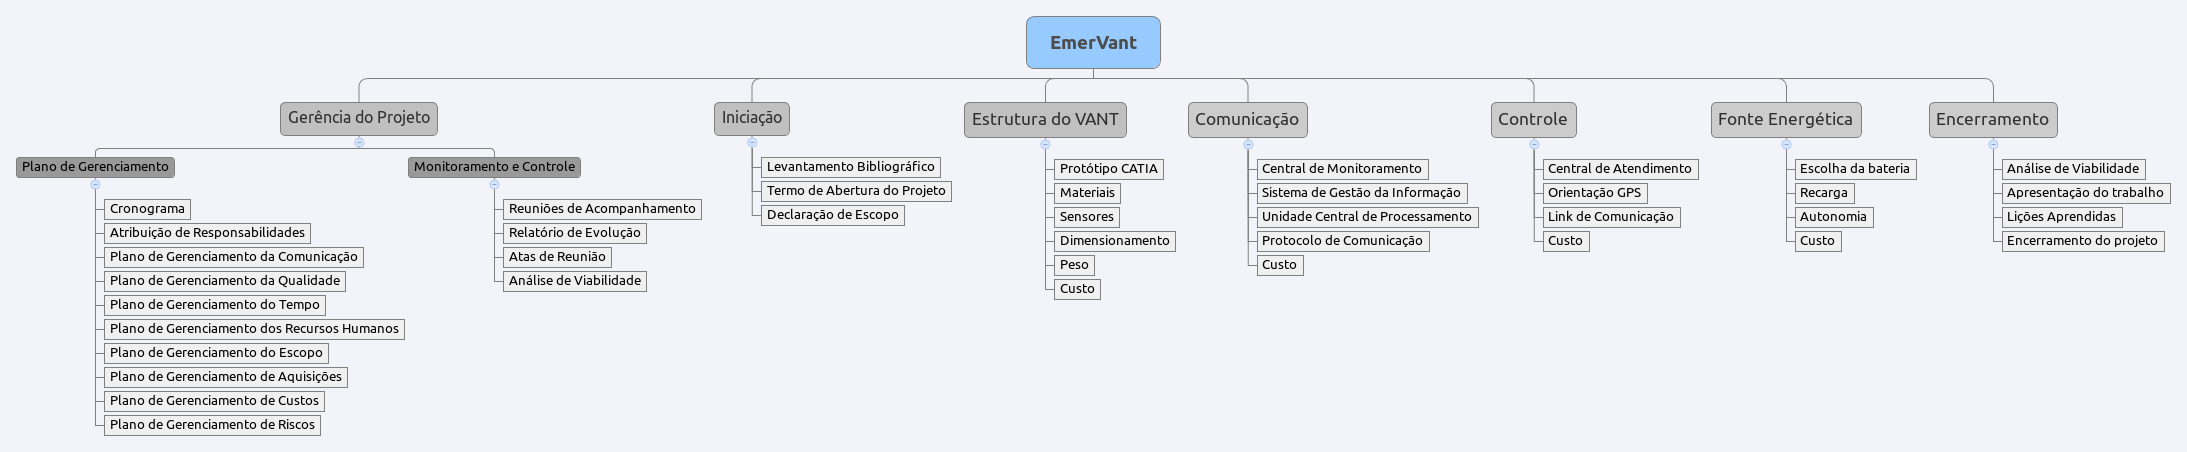
\includegraphics[height=6cm,width=16cm]{figuras/eap.eps}
  \caption{Estrutura Analítica do Projeto EmerVant}
  \label{fig:eap}
\end{figure}
\vfill
\pagebreak
